%%%%%%%%%%%%%%%%%%%%%%%%%%%%%%%%%%%%%%%%%%%%%%%%
\input{preamble.ltx}

% correct bad hyphenation here; separate each word by a space
\hyphenation{op-tical net-works semi-conduc-tor}

%%%%%%%%%%%%%%%%%%%%%%%%%%%%%%%%%%%%%%%%%%%%%%%%
\begin{document}

\title{BLUETOOTH and WIFI-ENABLED PANIC BUTTON for POTENTIAL RAPE VICTIMS} %ang imomodify daw yung BLUETOOTH and WIFI

\author{
	{\small
		%\renewcommand{\arraystretch}{1.3}
		\begin{tabular}{l l l}
			& \multicolumn{2}{c}{\tiny \textcolor[rgb]{0.9,0.9,0.9}{Participated in \& did the coursework [Y/N]?}} 
			\\ 
			GUEVARRA,~Alnair~M.~(11524855) & Y & 
\includegraphics[height=5ex] {A_signature} 
			\\ 
			HERNANDEZ,~Roy~Stephen~A.~(11530731)     & Y & %\includegraphics[height=5ex]{JDC_signature}
			\\ 
			LAGMAN,~Maria~Josefa~M.~(11531029)  & Y & 
\includegraphics[height=5ex]{mama_signature} 
			\\
			MOLINA,~Adam~M.(11539607)  & Y & %\includegraphics[height=5ex]{Capture1}
			\\  		
		\end{tabular}
	}
% for author names; note positions of commas and nonbreaking spaces ( ~ ) LaTeX will not break a structure at a ~ so this keeps an author's name from being broken across two lines.
\thanks{\CrmD\protect\\} %<--Do not delete this \thanks{\CrmD\protect\\} 
 \thanks{Coursework Starting Date: \hspace{1ex} July 13, 2018}
\thanks{Submission Date: \hspace{1ex} August 18, 2018}} 

\markboth{\makebox[\columnwidth]{DIGCOMM Project \hfill}%
\hspace{\columnsep}\makebox[\columnwidth]{\hfill}}%
{} % header

\IEEEpubid{\makebox[\columnwidth]{DIGCOMM - EK \hfill DLSU}%
\hspace{\columnsep}\makebox[\columnwidth]{ \hfill {\tiny\textcolor[rgb]{0.4,0.4,0.4}{\prsDy}}}} % footer

\maketitle % for making the title area


\section{Conspectus}
\label{sec:cnspcts}

\IEEEpubidadjcol % needed in second column of first page if using \IEEEpubid

\subsection{What are the objectives of the coursework?}
\begin{enumerate}
	\item To assess any Digital Communications Technology (DCT) to be used in marginalized sector.
	\item To modify the DCT appropriate to the selected marginalized sector.
	\item To appraise the economic, societal, and environmental implications of the modified DCT.
\end{enumerate}	

\subsection{How does the coursework fit with the course and previously done coursework?}
By:
\begin{enumerate}
	\item Involving the creation of a communication platform between caregivers and the elderly in case of emergencies.
	\item Using communications technology to notify app users immediately when the panic button is pressed.
\end{enumerate}	

\subsection{How were the objectives achieved?}
By:
\begin{enumerate}
	\item Targeting the marginalized sector of the DCT which is the elderly
	\item Implementing an additional mode of addressing an emergency via communications app
\end{enumerate}

\subsection{What are the key results and generalizations?}
The key results are:
\begin{enumerate}
	\item The modification of the bandpass modulation part in the GSM module
	\item The effective communication between the GSM module and the emergency contact number
\end{enumerate}

\section{Concepts and Principles}
\label{sec:concps}

\subsection{What are the necessary and relevant concepts and principles for understanding the coursework and for supporting the correct results?}
\begin{enumerate}
	\item A good understanding about Android application development 
	\item Knowledge about proper hardware input detection with bluetooth devices.
	
\end{enumerate}

\subsection{How does any new component, not covered in  previous coursework, function?}
By:
\begin{enumerate}
	\item Adding an online emergency notification to linked personal devices
	\item Implementing an automatic emergency hotline dialling on panic-button press
\end{enumerate}


\subsection{What figures, equations, and/or tables could support your answers in Sec. 2.1 and Sec.2.2?}
\begin{enumerate}
	\item Up to two lines per item. Figure \ldots shows \ldots
	\item Up to two lines per item. Table \ldots shows \ldots
\end{enumerate}

\subsection{Did you cite more than two publications in your answers in Sec. 2.1. and 2.2}
No.
	
\subsection{Did you cite any online source in your answers in Sec.2.1 and Sec.2.2?}
No.


\section{Methodology}

\subsection{How does your implementation in Sec.~\ref{sec:implem} achieve the objectives?}
By:
\begin{enumerate}
	\item Up to two lines per item.
	\item Up to two lines per item.
\end{enumerate}

\subsection{Why does your implementation in Sec.~\ref{sec:implem} achieve the objectives?}
Because:
\begin{enumerate}
	\item Up to two lines per item.
	\item Up to two lines per item.
\end{enumerate}

\subsection{How does your evaluation in Sec.~\ref{sec:eval} achieve the objectives?}
By:
\begin{enumerate}
	\item Up to two lines per item.
	\item Up to two lines per item.
\end{enumerate}

\subsection{Why does your evaluation in Sec.~\ref{sec:eval}  achieve the objectives?}
Because:
\begin{enumerate}
	\item Up to two lines per item.
	\item Up to two lines per item.
\end{enumerate}



\subsection{Implementation}
\label{sec:implem}

Rule of thumb: Implementation is how you made your  work; (keywords: implemented, created, made, soldered, programmed, etc.).


\subsubsection{What were the materials used?}
If the presentation would be better and necessary, tabulate your answers here instead of enumeration.
\begin{enumerate}
	\item Up to two lines per item.
	\item Up to two lines per item.
\end{enumerate}


\subsubsection{What is the summary of the processes used to make the coursework?}
If you wrote a program or made a simulation, you must add statements how the program or simulation functions in this section.	A pseudocode as shown in Table~\ref{tab:calcxn} is a good example.
\begin{enumerate}
	\item Up to two lines per item.
	\item Up to two lines per item.
\end{enumerate}

\begin{table}[!b]
	\caption{Pseudocode for the calculation of $y = x^n$}
	\label{tab:calcxn}	
	\centering
	{\footnotesize
		\begin{tabular}{lll}
			\hline
			\hline
			{\bfseries Input(s):} & & \\
			$n$ & : & $n$th power; $n \in \mathbb{Z}^{+}$ \\
			$x$ & : & base value; $x \in \mathbb{R}^{+}$ \\
			\hline
			{\bfseries Output(s):} & & \\
			$y$ & : & result; $y \in \mathbb{R}^{+}$  \\
			\hline
			\hline
			\\
		\end{tabular}
	}
	\begin{algorithmic}[1]
		{\footnotesize
			\REQUIRE $n \geq 0 \vee x \neq 0$
			\ENSURE $y = x^n$
			\STATE $y \Leftarrow 1$
			\IF{$n < 0$}
			\STATE $X \Leftarrow 1 / x$
			\STATE $N \Leftarrow -n$
			\ELSE
			\STATE $X \Leftarrow x$
			\STATE $N \Leftarrow n$
			\ENDIF
			\WHILE{$N \neq 0$}
			\IF{$N$ is even}
			\STATE $X \Leftarrow X \times X$
			\STATE $N \Leftarrow N / 2$
			\ELSE[$N$ is odd]
			\STATE $y \Leftarrow y \times X$
			\STATE $N \Leftarrow N - 1$
			\ENDIF
			\ENDWHILE
		}
	\end{algorithmic}
\end{table}







\subsection{Evaluation}
\label{sec:eval}

Rule of thumb: Evaluation is how you tested your  work for correctness; (keywords: measured, tested, compared, simulated, etc.).

\subsubsection{What were your procedures for evaluating the correct outcome of your coursework?}
\begin{enumerate}
	\item Up to two lines per item.
	\item Up to two lines per item.
\end{enumerate}

\subsubsection{What quantities were gathered and how have you obtained them for testing the veracity of your results?}
\begin{enumerate}
	\item Up to two lines per item.
	\item Up to two lines per item.
\end{enumerate}


\section{Results and Discussions}

\subsection{How do the results achieve the objectives?}
By:
\begin{enumerate}
	\item Up to two lines per item.
	\item Up to two lines per item.
\end{enumerate}

\subsection{Why do the results achieve the objectives?}
Because:
\begin{enumerate}
	\item Up to two lines per item.
	\item Up to two lines per item.
\end{enumerate}

\subsection{Are all you results correct  in accordance to what you described in Sec.~\ref{sec:eval} evaluation process? Why?} 
Yes/no, because:
\begin{enumerate}
	\item Up to two lines per item.
	\item Up to two lines per item.
\end{enumerate}

\subsection{What is result $X$ (briefly describe it here), what does it mean if it is correct, and how does it contribute in reaching the objectives?}
\label{sec:resn}

\begin{enumerate}		
	\item Refer to the appropriate caption number  of your result, i.e. Fig.~$X$ for figure $X$, Table~$X$ for table $X$, etc.	
	\item Interpret result $X$ and the reasons why it was obtained. 
	
	\item Point out and explain apparent discrepancies from principles/concepts/theory if your result is incorrect.
	
	\item Cite existing publication for comparison of your result.
	
	\item Do not present your result as ``It worked'' without an appropriate explanation as such action does not show thorough understanding.
	
	
	\item Repeat Sec.~\ref{sec:resn} for each major result $X$ (i.e. $X$=1, $X$=2, etc.).		
\end{enumerate}

For example, result $X = 1$ (on the accuracy performance of the enhanced bi-directive method):

\begin{enumerate}
	\item Figure \ldots shows that the performance of the system is satisfactory up to 90\%.
	\item The result in Figure \ldots was obtained because of the bi-directive mechanism of the proposed architecture.
	\item The remaining 10\% accuracy loss is due to the failure of the bi-directive mechanism to \ldots and supported by \ldots.
	\item Reference~\cite{Einstein1905} also achieved similar range of results from 85\% to 93\%.
	\item \ldots
\end{enumerate}

\subsection{Did you cite more than two publications in your answers above (yes/no)?}
Yes.	



















\section{Conclusions}
\label{sec:conc}

\subsection{What are the main points that should be known, remembered, and learned about the coursework?}
\begin{enumerate}
	\item Up to two lines per item.
	\item Up to two lines per item.
\end{enumerate}

\subsection{What are the gists of the inferences drawn from your results?}
\begin{enumerate}
	\item Up to two lines per item.
	\item Up to two lines per item.
\end{enumerate}

\subsection{Briefly, what are your comments on (1)~your results, and  (2)~future coursework if any?}
\begin{enumerate}
	\item Up to two lines per item.
	\item Up to two lines per item.
\end{enumerate}	


\bibliographystyle{IEEEtr}
\bibliography{references} % references section

\newpage
\begin{figure*}[!t]
	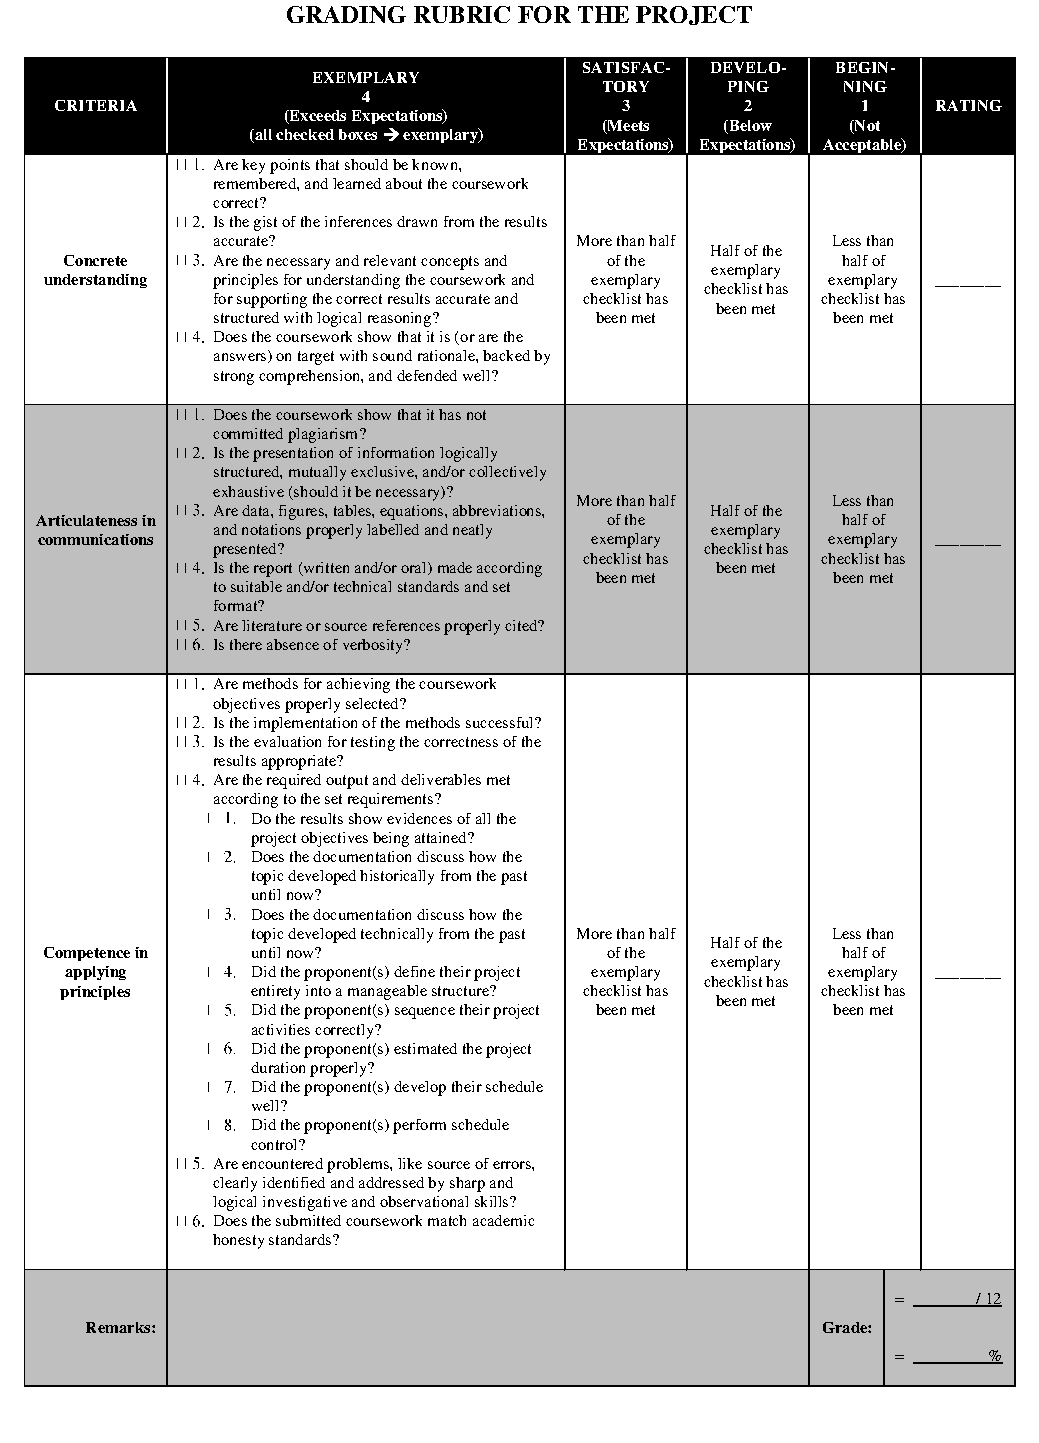
\includegraphics[width=\textwidth]{rubric} 
\end{figure*}
\cleardoublepage

\end{document}